\documentclass[11pt]{article}
\usepackage[utf8]{inputenc}
\usepackage[margin=1in]{geometry}
\usepackage{enumitem}
\usepackage{titlesec}
\usepackage{graphicx}
\usepackage{xcolor}              % Color mixing (e.g., blue!70!black)
\usepackage{hyperref}
\usepackage{charter}           % Charter font
\usepackage{microtype}         % Improved typography
\usepackage{setspace}          % Line spacing control
\usepackage{parskip}           % Better paragraph spacing
\usepackage[font={small,color=gray}]{caption}  % Smaller, gray captions

% Hyperlink styling
\hypersetup{
    colorlinks=true,
    linkcolor=black,
    urlcolor=blue!70!black,
    citecolor=black
}

% Custom section formatting with spacing
\titleformat{\section}{\Large\bfseries}{\thesection}{1em}{}[\titlerule]
\titlespacing*{\section}{0pt}{2em}{1em}

% Figure spacing
\setlength{\intextsep}{1.5em}
\setlength{\floatsep}{1.5em}
\setlength{\textfloatsep}{2em}

\begin{document}

% ==================== COVER PAGE ====================
\begin{titlepage}
    \centering
    \vspace*{2cm}
    
    {\Large\textsc{The Pennsylvania State University}}\\[0.3cm]
    {\large\textsc{Multi-campus REU Program}}\\[2cm]
    
    \rule{\textwidth}{1.5pt}\\[0.5cm]
    {\LARGE\bfseries Monte Carlo Radiative Transfer Beaming Functions for NICER Pulse-Profile Modeling}\\[0.5cm]
    \rule{\textwidth}{1.5pt}\\[2cm]
    
    {\Large\textbf{Research Proposal}}\\[3cm]
    
    \begin{tabular}{rl}
        \textbf{Student Name:} & Ameya Panchal \\[0.5em]
        \textbf{Penn State ID:} & avp6407 \\[0.5em]
        \textbf{Project Campus:} & University Park \\[0.5em]
        \textbf{Project Start Date:} & January 2026 \\[0.5em]
        \textbf{Primary Faculty Mentor:} & Dr. Asif Ud-Doula \\[0.5em]
        \textbf{Mentor Affiliation:} & Penn State Scranton \\[0.5em]
        \textbf{Mentor Email:} & auu4@psu.edu \\
    \end{tabular}
    
    \vfill
    
    {\large February 2026}
    
\end{titlepage}

% ==================== MAIN CONTENT ====================
\setstretch{1.15}

\section*{Project Overview and Motivation}
Neutron stars are some of the strangest objects in the universe. They are only about the size of a city, but they pack more mass than the Sun, spin hundreds of times per second, and produce powerful beams of radiation that we can detect from Earth. I am interested in studying how this radiation is produced and how we can use it to learn more about the fundamental properties of neutron stars.

During the MC REU program, I would like to work on a research project that focuses on how radiation escapes from the surface of a neutron star and how that radiation appears to observers using NASA's NICER telescope aboard the International Space Station. NICER measures X-rays from rapidly spinning neutron stars (called pulsars), and scientists use these observations to estimate the star's mass and radius. These measurements help answer big questions about the nature of matter at extremely high densities—conditions that cannot be recreated in laboratories on Earth.

One important challenge in this process is understanding how radiation actually leaves the neutron star's surface. Most models assume that the radiation comes out evenly in all directions, but this may not be realistic. The surface layers of a neutron star are extreme environments, where photons scatter many times before escaping. This scattering can cause the radiation to be beamed more strongly in certain directions, which directly affects what NICER observes as the star rotates.

\vspace{1em}
\begin{figure}[htbp]
    \centering
    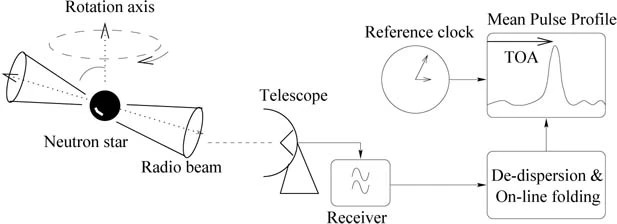
\includegraphics[width=0.65\textwidth]{descriptive_image.png}
    \caption{Illustration of a rotating neutron star and the resulting X-ray pulse profile observed by telescope (Lorimer).}
\end{figure}
\vspace{0.5em}

This project aims to model how the shape of this pulse changes based on atmospheric scattering.

\vspace{1em}
\begin{figure}[htbp]
    \centering
    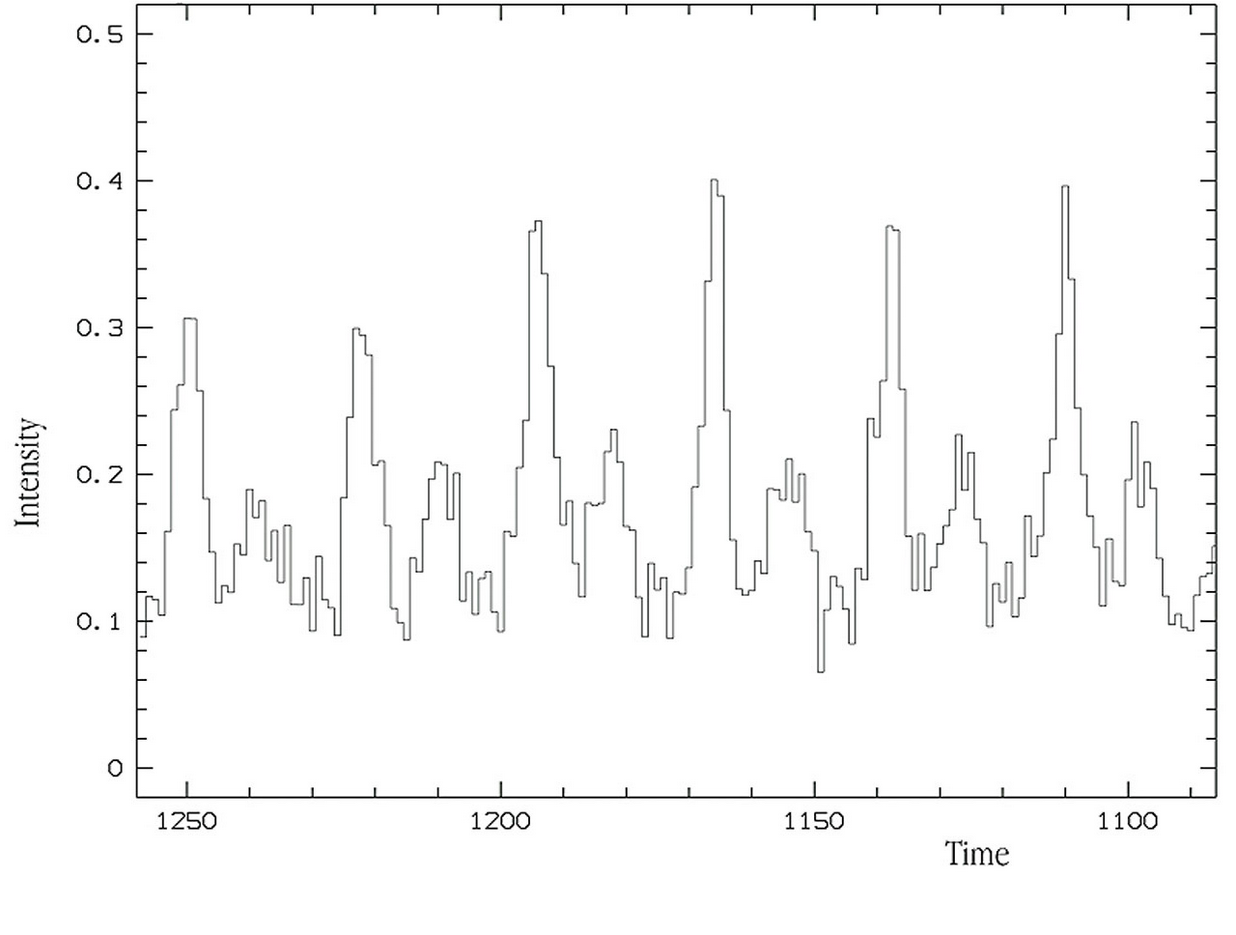
\includegraphics[width=0.65\textwidth]{graph.png}
    \caption{A schematic of a neutron star pulse profile (Light Curve). The graph shows Intensity (Y-axis) varying with Time (X-axis) as the star rotates and the hot spot sweeps past the observer (eso).}
\end{figure}
\vspace{0.5em}

My project will simulate these curves to see how they change when realistic atmospheric scattering is included.

\newpage
\section*{Scientific Significance}
Understanding neutron stars is one of the most important frontiers in modern physics. Neutron stars contain matter compressed to two or three times the density of an atomic nucleus—conditions so extreme that they cannot be recreated in any laboratory on Earth. By measuring the mass and radius of neutron stars, scientists can determine how matter behaves under these extreme pressures, a relationship known as the ``equation of state'' of dense matter. This is a fundamental question in nuclear physics that connects to our understanding of the strong nuclear force.

NASA's NICER telescope uses a technique called Pulse Profile Modeling to measure neutron star masses and radii with unprecedented precision. However, this method relies on assumptions about how radiation escapes from the surface. If these assumptions are incorrect, the inferred masses and radii may be biased. My project addresses this directly: by simulating realistic atmospheric scattering, I can provide improved beaming functions that may help reduce systematic uncertainties in NICER's measurements. Even small improvements in modeling could refine our understanding of the fundamental physics governing the densest matter in the universe.

\section*{Proposed Methodology}
My proposed project is to model this process using a Monte Carlo simulation. In simple terms, this means I will simulate millions of individual "photon packets" as they move through a thin layer above the neutron star's surface. Each photon travels a short distance, scatters off a particle, and changes direction.

By tracking the directions in which these photons finally escape, we can determine the surface brightness as a function of angle (the "beaming function"). Once the beaming function is calculated, it can be used to generate synthetic pulse profiles. These profiles will be compared to simpler models to see how much the assumed physics of the surface affects our interpretation of NICER data. Specifically, I will look at how the "pulsed fraction" (how much the brightness changes as the star spins) is influenced by different scattering scenarios.

\section*{Research Timeline (10 Weeks)}
\begin{itemize}[leftmargin=*]
    \item \textbf{Weeks 1--2: Literature Review and Physics Setup.} I will spend the first two weeks reading core papers on NICER and the physics of Thomson scattering. I will also set up the development environment for the simulation (using Python or C).
    \item \textbf{Weeks 3--5: Developing the Monte Carlo Engine.} I will write the code to simulate photon packets being injected and scattering within a model atmosphere. I will validate the code by ensuring it conserves energy and correctly handles random walks.
    \item \textbf{Weeks 6--7: Extracting the Beaming Function.} I will run the simulation many times to get high-quality statistics. I will then bin the escaping photons by their exit angle to create a beaming function.
    \item \textbf{Weeks 8--9: Pulse Profile Generation.} I will combine the beaming function with a geometric model of a spinning star to create synthetic light curves, taking into account basic relativistic effects like light bending.
    \item \textbf{Week 10: Analysis and Final Report.} I will compare my results to standard models and write a final report summarizing how different atmospheric conditions change what a telescope like NICER would see.
\end{itemize}

\section*{Impact and Personal Goals}
This project allows me to apply computational physics to a real-world problem in a very direct way. The simulations are conceptually simple but physically meaningful, and the results can be compared to real astronomical data. Even modest changes in the beaming pattern can noticeably change the predicted pulse profiles, meaning this work can help reduce uncertainties in how neutron star properties are inferred from NICER observations.

This project is also well suited to my background and interests. It will allow me to develop strong computational skills, learn how Monte Carlo simulations are used in astrophysics, and gain experience working on a problem that is relevant to current research. I am especially motivated by the possibility that this work could lead to a short refereed journal publication, which would be an invaluable experience as I consider pursuing graduate studies in physics or astronomy.

\section*{Qualifications}
I am well-prepared for this project. Since Fall 2025, I have been conducting independent research on Monte Carlo simulations at Penn State, developing computational models in Python to simulate probabilistic systems and analyzing experimental data using machine learning tools. As a Computer Science major with a Physics minor in the Schreyer Honors College, I have both the programming expertise to implement complex simulations and the physics foundation to understand the underlying scattering processes.


\section*{Plan for Engagement}
\begin{itemize}[label=\textbullet]
    \item \textbf{Weekly Meetings:} Scheduled 1-hour in-person or Zoom calls with Dr. Asif ud-Doula to review code, discuss physics obstacles, and set weekly goals.
    \item \textbf{Collaboration:} All code will be hosted on a private GitHub repository, allowing for asynchronous code review and progress tracking.
    \item \textbf{Mid-Summer Check-in:} A dedicated review at Week 5 to validate the Monte Carlo engine against analytical benchmarks before proceeding to the pulse profile generation.
\end{itemize}

\section*{References}
\noindent Lorimer, D.R. Binary and Millisecond Pulsars at the New Millennium. Living Rev. Relativ. 4, 5 (2001). \url{https://doi.org/10.12942/lrr-2001-5}

\noindent \url{https://www.eso.org/public/images/eso9948i/}

\end{document}